% ----------------------------------------------------------------------------------------------------------------------------------
% Document Preamble
% ----------------------------------------------------------------------------------------------------------------------------------
\documentclass[11pt, A4]{article}

% Packages and formatting
\usepackage[utf8]{inputenc}
\usepackage{times}
\usepackage{blindtext}
\usepackage{float}
\usepackage[labelfont=bf, font={scriptsize,sf}, format=plain, indention=0em, margin=1em]{caption}
\usepackage[font={scriptsize,sf}]{subcaption}
\usepackage{geometry}
	\geometry{
 		a4paper,
% 		total={170mm,257mm},
 		left=15mm,
		right=15mm,
 		top=20mm,
		bottom=30mm,
	}
\usepackage{multicol}
	\raggedcolumns
	\raggedbottom
	\setlength{\columnsep}{2em}
\usepackage{datetime}
	\newdateformat{monthyeardate}{\monthname[\THEMONTH], \THEYEAR}
\usepackage{graphicx}
	\graphicspath{ {./images/}}
\usepackage{fancyhdr}
	\renewcommand{\headrulewidth}{0.5pt}
	\fancyhead[R]{
		\includegraphics[width=6cm]{mpi-logo.png}
	}
	\pagestyle{plain}
\newenvironment{Figure}
  {\par\medskip\noindent\minipage{\linewidth}}
  {\endminipage\par\medskip}





% Title definitions
\title{Modelling The Activity of MBONs Based On DAN Activity In The Drosophila Mushroom Body}
\author{Jake Pencharz, Shuai Shao, Julijana Gjorgjieva}
\date{\monthyeardate \today}   


% ----------------------------------------------------------------------------------------------------------------------------------
% Begin Document
% ----------------------------------------------------------------------------------------------------------------------------------
\begin{document}
\raggedbottom
\raggedcolumns

% Place title
\maketitle

\thispagestyle{fancy}
% Multi-columns
\begin{multicols}{2}


% ==== Abstract ====
\begin{abstract}
The Mushroom Body (MB) is established as a site for associative learning in insects. The structure is split into 15 compartments, demarcated by the presence of specific mushroom body output neurons (MBONs), and dopaminergic neurons (DANs). Each of these compartments provides a site for parallel learning. Dopamine has been shown to convey essential information about the valence of odours to each of these compartments. Similarly it has been shown that MBONs use this valency information in their representation of odours to initiate an appropriate behavioural response. We sought to model the relationship between DANs and MBONs. Several models are investigated ranging from a simple one-to-one linear model to a recurrent model where MBONs feed back into the MB compartments. Given that the connectome of the Drosophila Melanogaster MB has recently become available, the models' learned weights are compared with these known synaptic connections. 
\end{abstract}

% ==== Introduction ====
\section{Introduction}
The Drosophila Melanogaster is a useful model for understanding how memories are formed and used to influence behaviour. Fruit flies can learn to approach odours which have previously been paired with food, and avoid those paired with shock \cite{aso2014neuronal}. Clearly these responses are not purely innate but can be learned. It is well established that the Mushroom Body (MB) is the major site of associative learning in insects. This brain structure learns to integrate past information and current sensory stimuli to inform decision making. 

More specifically, the MB has been widely implicated as the structure which translates olfactory information to a behavioural response. Unlike most other structures in the insect brain, the MB  is not completely predetermined. The Kenyon Cells (KCs), whose projections form the bulk of the MB, do not receive stereotyped inputs from the olfactory projection neurons. The MB is therefore required to to learn how to interpret this abstract representation of odour, and use it to induce an appropriate behaviour. The MB may therefore represent an evolutionary primitive brain structure similar in form and function to structures in the vertebrate brain. A deeper understanding of how learning occurs in the MB could, therefore, provide insight into higher associative functions in vertebrate brains. 

The MB is split into 15 compartments  \cite{aso2014neuronal, li2020connectome} based on the characteristic distribution of Mushroom Body Output Neurons (MBONs). Within each compartment the MBONs form synapses with the axons of the KCs within the MB. The strength of these synapses is strongly affected by the presence of Dopaminergic Neurons (DANs). These DANs allow each compartment to act as a separate unit of memory formation and associative learning. Associative memories are therefore stored as changes to the strength of the synaptic connections between the KCs and their target MBONs. 

For decision making, the pathways which convey sensory information, must converge with the pathways that convey reward and punishment. This is precisely what occurs when information from the KCs and the DANs reach a MBON. In both vertebrates and invertebrates, dopamine plays an important role in conveying valence of a stimulus \cite{li2020connectome}. Therefore the activity of the DANs conveys the valence of a stimulus to the MBONs. The MBONs, which project into a variety of external brain areas, use this valence information to influence the fly's behavioural response to an odour. 

 Since the DANs convey valence, and that ultimately informs the fly's response to an odour, it may therefore be possible to predict the activity in the MBONs given only the activity of the DANs. The following paper presents an investigation of different models used to predict MBON activity from DAN activity. As well as the predictive power of the models, their efficacy is quantified by comparing their learned  parameters to the known connectome of the Drosophila MB \cite{li2020connectome}.



% ==== Structure and Functions of the Mushroom Body ====

\begin{figure*}[t]
	\centering
	\includegraphics[width=\textwidth]{siju-mb.png}
	\caption{Figure taken from Siju 2020 illustrating the basic structure of the MB and the MB compartments. \textbf{c} indicates the complex interconnected structure of the MB which arises due to feedback between the different cell types.}
	\label{fig:siju-mb}
\end{figure*}

\section{Background To This Study}

The structure of the MB allows it to perform associative learning. Through drastic dimensionality reduction, and input from the DANs the odour identity encoded by the KCs is transformed into information about the valence of the odour.

The input to the MB comes from the antennal lobe which maintains a topographic map of olfactory stimuli. However, since the projections from the antennal lobes to the KCs are not stereotyped, this topographic map is lost when it projects to the KCs. The KCs form a sparse  (only a small percentage of KCs are activated by an odour) representation of this information which encodes the identity of the odour.

		
neuropil
The MB is a neuropil comprising of the 2200 KC axons \cite{aso2014neuronal}. There are three classes of KCs which split the MB into three distinct lobes $\alpha /\beta$, $\alpha' /\beta'$ and $\gamma$. Due to their orientation, it is common to refer to  
$\beta, \beta' $, and $\gamma$ lobes as the medial/horizontal lobes and the $\alpha, \alpha'$ lobes as the vertical lobes. There are seven Kenyon Cell types whose parallel fibres further subdivided the lobes into layers:

\begin{itemize}
\itemsep0pt
\item  $\alpha /\beta$ - divided into 3 layers posterior (p), core(c), and surface(s)
\item $\alpha' /\beta'$ - divided into 2 layers: middle (m) and anterior-posterior (ap)
\item  $\gamma$ - divided into 2 layers: main and dorsal (d)
\end{itemize}


Within the lobes, the dendrites of MBONs and projections of DANs overlap with the KC axons. There are 22 typical types of MBON cells,  and an additional 14 atypical MBON types whose dendrites extend out of the MB  \cite{li2020connectome}. Furthermore, there are approximately 20 DAN types which innervate the MB. The presence of particular MBONs and DANs form anatomical subdivisions, the MB compartments, which are considered the units of associative learning. %%%%
% [(Aso et al., 2012; Aso et al., 2010; Aso et al., 2019; Aso et al., 2014a; Aso et al., 2014b; Aso and Rubin, 2016; Berry et al., 2018; Blum et al., 2009; Bouzaiane et al., 2015; Burke et al., 2012; Claridge-Chang et al., 2009; Isabel et al., 2004; Jacob and Waddell, 2020; Krashes et al., 2009; Lin et al., 2014b; Liu et al., 2012; Owald et al., 2015; Pai et al., 2013; Perisse et al., 2016; Qin et al., 2012; Plac ̧ ais et al., 2013; Schwaerzel et al., 2003; Se ́ journe ́ et al., 2011; Trannoy et al., 2011; Yamagata et al., 2015; Zars et al., 2000)](). In general it has been found that synaptic depression between the MBONs and KCs occurs when the KCs co-activate with DANs in a particular compartment [(Hige 2015)]().
 %%%

Importantly, the MB performs a form of dimensionality reduction, compressing the information carried by around 2000 KCs to something on the order of 30 MBONs. The activation of MBONs no longer encodes odor identity, but is rather tuned towards generating particular behaviours. In fact \cite{hige2015} found that the full set of MBON activations is tuned to the valence of particular stimuli (see Figure \ref{fig:odor-clusters-mb}). 

\begin{figure}[H]
	\centering
	\includegraphics[width=0.9\linewidth]{odor-clusters-mb.png}
	\caption{Figure taken from Hige 2015 illustrating the change in odor representation that occurs between KCs and MBONs. In the KCs the odour identities are easily separated out. However the MBONs distinguish between the valence of the odour rather than its identity. This is useful for informing behaviour downstream from the MB.}
	\label{fig:odor-clusters-mb}
\end{figure}


Genetic manipulation has implicated specific subsets of MBONs in the mediation of learned appetitive and aversive behaviours 
%([Sejourne et al., 2011](https://elifesciences.org/articles/04577#bib86); [Pai et al., 2013](https://elifesciences.org/articles/04577#bib70); [Placais et al., 2013](https://elifesciences.org/articles/04577#bib77); [Aso et al., 2014](https://elifesciences.org/articles/04577#bib4)).
 These experiments implicate the DANs as the source of the learning cue and the MBONs as the mediators of behavioural output.


% ==== MBONs====
\subsection{MBONs}

14 MBON cell types have 1 cell per hemisphere while six types have two cells and one type has eight cells (MBON-$\beta'$ 1 which is GABAergic). The MBONs can also be characterised by the type of neurotransmitter that they release:

\begin{itemize}
\itemsep0em
\item Eight cholinergic cell types. These are found in the $\alpha, \alpha '$ (vertical) lobes
%
\item Seven glutaminergic cell types found in  the $\beta, \beta', \gamma$ (medial/horizontal) lobes
%
\item Four GABAergic cell types found mainly at the intersection between the horizontal and vertical lobes
\item Two other types
\end{itemize}


Usually, the dendrites from each MBON arborise in a single compartment. However eight of the MBON cell types have dendrites which extend into two compartments.

Usually the dendrites span layers within the lobe (ie they arborise to all the KCs present in all layers of that compartment). However, 8 cell types restrict their connections to a single layer (see Figure \ref{fig:mbons_per_lobe}).


% ==== DANs ====
\subsection{DANs}
There are around 130 DANs of 20 different types. Different populations of DANs activate based on the valence of an odor: PPL1 DANs convey negative valence, and PAM neurons convey positive valence. These populations project into the MB conveying either reward or punishment signals to facilitate learning. 17 out of the 20 DAN cell types only project into a single MB compartment.

The MB structure causes the different MBON types to have access to largely equivalent input from the KCs. However, each compartment and hence almost every MBON cell type, receives unique information from unique sets of DANs. In classical learning paradigms, different DAN types respond to different unconditioned stimuli (US). Therefore the MBON activation depends on the DAN's response to a stimulus and thus the DANs convey valence information about the US to specific MBON types. Dopamine release in specific compartments modifies local KC–MBON synapses to bias behavioural output. This relationship implies that it may be possible to predict MBON behaviour given the response of the DAN population in the MB. 


% ==== MBON Feedforward Network ====
\subsection{MBON Feedforward Network}

The DANs and KCs are not the only inputs to the MBONs. A few of the MBON cell types, as well as projecting outside of the MB structure, project back into other compartments of the MB. This creates a multilayer feedforward network:

\begin{enumerate}
\item
Layer 1 consists of MBON cells types which exclusively receive input from the KCs. These reside mostly in the $\alpha'; \beta'; \gamma$ lobes. This set includes  (MBON-$\gamma 4> \gamma 1 \gamma2$) which feeds forward from $\gamma 4$ to cells in compartments $\gamma 1$ and $\gamma 2$. 
%
\item
The second layer of the network comprises MBON cells in $\gamma 1$ and $\gamma 2$ receiving input from KCs and the $\gamma 4$ compartment. These include (MBON-$\gamma 1pedc > \alpha / \beta$) which feeds forward to the third layer.
%
\item
The third layer of MBON cells has dendrites in the $\beta1, \beta2$ compartments. The projections from the $\gamma 1pedc$ compartment affect their activity. These cells include  (MBON-$\beta 1 > \alpha$) which feeds forward to the fourth and final layer
%
\item
MBON cells in the $\alpha$ lobe therefore have access to information passed on to them from many of the MB compartments via the three preceding layers.
\end{enumerate}


It can be argued that this layering increases the computational capacity of the network providing an efficient mechanism for modifying and updating previous learnings.


\begin{table*}[t]
\begin{center}
\begin{tabular}{l | l | r | r | r | r }
\hline
Stimulus & Valence & Total Trials & Virgin Trials  & Fed Trials & Common \\
\hline
3Octanol        &  negative & 17.0 &  17.0&  8 & yes \\
4MCH             & negative & 22.0 &22.0& 11 &  yes \\
Citronella        & negative & 49.0 & 49.0&  11 &yes \\
Peppermint       & negative &25.0 & 25.0&  12 & yes \\
Vinegar           & positive & 42.0 & 42.0&  11 & yes \\
Yeast            & positive & 45.0 & 45.0 & 14 &yes \\
1-Hexanol      & unknown &   20.0 &    20.0 & 8 &   yes \\
2-Heptanone & unknown &      21.0 &      21.0& 9 &  yes \\
Ethanol           & unknown &13.0 & 13.0&  6 &yes \\
Geosmin         & negative &  15.0 & 15.0& 9&  no \\
Isoamylacetate & unknown &   25.0 & 25.0& 12& no \\
cVA              & unknown & 68.0 & 38.0 & 68  & no \\
\hline
\end{tabular}
\end{center}
\caption{Summary of Siju 2020 dataset. The stimuli which are not common between the data from  \cite{siju2020} and \cite{hige2015} are not used in this study.}
\label{tab:siju_data}
\label{default}
\end{table*}%


% ==== Sources of Recurrence =====
\subsection{Sources of Recurrence}

There is one DAN cell type whose dendrites arborise within compartments $\gamma1; \gamma2$ and projects to $\gamma4$. This forms an internal recurrent loop within the MB where the regulatory effect of the DANs on  $\gamma4$ will be dependent on the activity in other MB lobes.

Another source of recurrence between the MBONs and DANs arises outside the MB. Many MBON projections converge to similar external structures in the brain. These projections overlap with the dendrites of DANs which innervate the MB. This allows for either positive or negative feedback between these two populations of cells. This negative feedback loop provides the opportunity for MBONs to suppress the activity of DANs, reducing the amount of learning that occurs once the correct response has been learned.

% ==== Data =====
\section{Data}
Two dataset from different studies,  \cite{siju2020} and  \cite{hige2015} are used to tune the models. The stimuli used in these two experiments are similar but not identical. 

Furthermore, both of the datasets are relatively small. Therefore it is required to increase the size of the dataset so that the data can be used to tune the weights of a generative model.

Several assumptions are made in cleaning and manipulating the raw data such that it can be used to optimise a computational model of the MB. 

% ==== DAN Data =====
\subsection{DAN Data}
The dataset from  \cite{siju2020} provides the activity of DANs in each of the MB compartments. Activity was recorded using two photon microscopy with calcium imaging. This dataset comprises of 393 total trials, where a trial corresponds to a single stimulus being presented and the activity from the 15 lobes being recorded.  The dataset was originally used to investigate the effect of starvation and virgin/ non-virgin states on the DAN response to odour stimuli. Therefore some flies were starved for either 24 or 48 hours, and some of the flies are mated. A summary of the dataset can be found in Table \ref{tab:siju_data} and for the relative activity in each of the compartments for each stimuli refer to Figure \ref{fig:siju-activity-per-stim}.



For comparative purposes only the data which was recorded from files in a similar manner to the data recorded by Hige is used. The stimulus set used in the two experiments are not identical. Therefore, there are 253 trials remaining after removing data generated using stimuli unique to the DAN dataset. From these only the un-starved flies are considered leaving 90 trials. For more details, see notebook \texttt{preprocess-siju.ipynb}.

		

% ==== MBON Data =====
\subsection{MBON Data}

To validate predictions made by the model, MBON activity data was supplied by \cite{hige2015}. This dataset contains 11 odor stimuli (including an 'empty' control). Nine of the 11 odours are common to the two datasets. There are therefore a total of 45 trials in the MBON dataset (see Table \ref{tab:hige_data}).

\begin{table}[H]
\begin{center}
\begin{tabular}{l | l | r | r  }
\hline
Stimulus & Valence & Total Trials & Common \\
\hline
octanol & negative & 5 & yes \\
mch	& negative & 5 & yes \\
citronella & negative & 5 & yes \\
peppermint & negative & 5 & yes \\
vinegar		& positive & 5 & yes \\
yeast 		 & positive &5 & yes \\
hexanol	& unknown & 5 & yes \\
2-heptanone & unknown & 5 & yes \\
ethanol & unknown &5 & yes \\
co2 & unknown & 5 & no \\
empty & none & 5 & no \\
\hline
\end{tabular}
\end{center}
\caption{Summary of Hige 2015 dataset. The stimuli which are not common between the data from Siju 2020 and Hige 2015 are not used in this study.}
\label{tab:hige_data}
\label{default}
\end{table}%


The activity triggered by these odours was recorded in 14 specific MBON cells of different types. In two cases the reading from a combination of two cell types is given. These two cases are ($\alpha'3ap \; \&\; m$) and ($\gamma3 \; \& \; \gamma3 \beta'1$). This dataset therefore covers 18 of the 21 MBON cell types.

\begin{figure}[H]
	\centering
	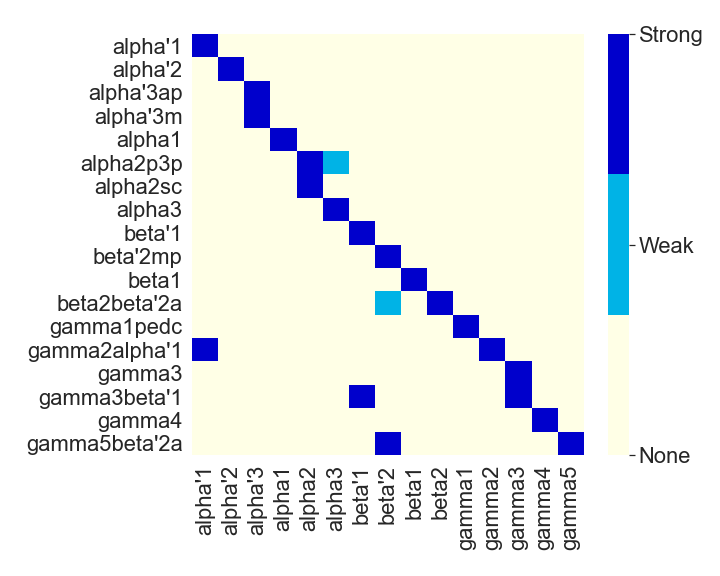
\includegraphics[width=\linewidth]{convert-cell-to-compartment.png}
	\caption{Mapping from MBON cell type (vertical axis) to MB compartment. Some of the MBON cells extend dendrites into more than one compartment and therefore their activity contributes to the activity in both of those compartments. A low dendritic presence qualifies as a weak mapping. The contribution of activity that this cell makes to the activity in the compartment is therefore weighted by 0,5.}
	\label{fig:convert-cell-to-compartment}
\end{figure}



The Siju dataset was not cell specific. Rather it was recorded as the activity per compartment of the MB. Therefore, for modelling purposes, it was required to translate the activity recorded from cells in the Hige dataset to an approximate activity per compartment of the mushroom body. This is mostly straightforward since MBON cell types are usually confined to a single compartment (in fact they delineate the compartments). For example the recorded activity of cell type $\alpha'1$ is considered to be the activity in the corresponding compartment. However, there are two cases where the conversion is not as straightforward: the combination recordings; and cell types which have dendrites in more than one compartment such as ($\gamma 2 \alpha'1$).

It is therefore assumed that, for each of the combination recordings, the activity contributed to each compartment is identical. Then, based on Figure 12 A in \cite{aso2014neuronal} the cell types are mapped to their corresponding compartment. If there is a small dendritic presence in a particular compartment, the contributed activity is weighted by 0,5. For details see Notebook \texttt{preprocess-hige-expanded.ipynb}.

		
	
% ==== Boosting =====
\subsection{Boosting the Dataset Size}

This study is interested in investigating the relationship between DANs and MBONs. Therefore an ideal dataset would consist of DAN measurements, and the resulting MBON measurement for a given odour. A model could then be fit to this ideal dataset to determine the relationship between these two groups of cells.

With only 90 trials for the DAN dataset, and 45 trials from the MBON dataset, it would not be possible to optimise a model and avoid over-fitting. Furthermore, since these two datasets were collected in isolation from one another, it is not possible to create a mapping from an input datum (a single DAN trial), and an output datum (a single MBON trial). 

To solve both of these problems the datasets were used to create sampling distributions. First, both datasets are normalised. For the DAN dataset, the data for each odor, and each of the 15 compartments is fit to a log-normal distribution (see Figures \ref{fig:dan-distribution} and \ref{fig:dan-distribution-all-stimuli}). The choice of distribution is based on the activity seen in each compartment across stimuli.

Similarly the MBON data is used to generate a normal distribution for each odor and each compartment in the MB (see Figures \ref{fig:mbon-distribution} and \ref{fig:mbon-distribution-all-stimuli}). For further details refer to the notebook \texttt{build-datadistributions.ipynb}.	


Using these distributions 27000 trials are generated (18000 training trials, and 4500 for both testing and validation).


\begin{figure*}
	\centering
	\begin{subfigure}[b]{0.49\textwidth}
		\centering
        		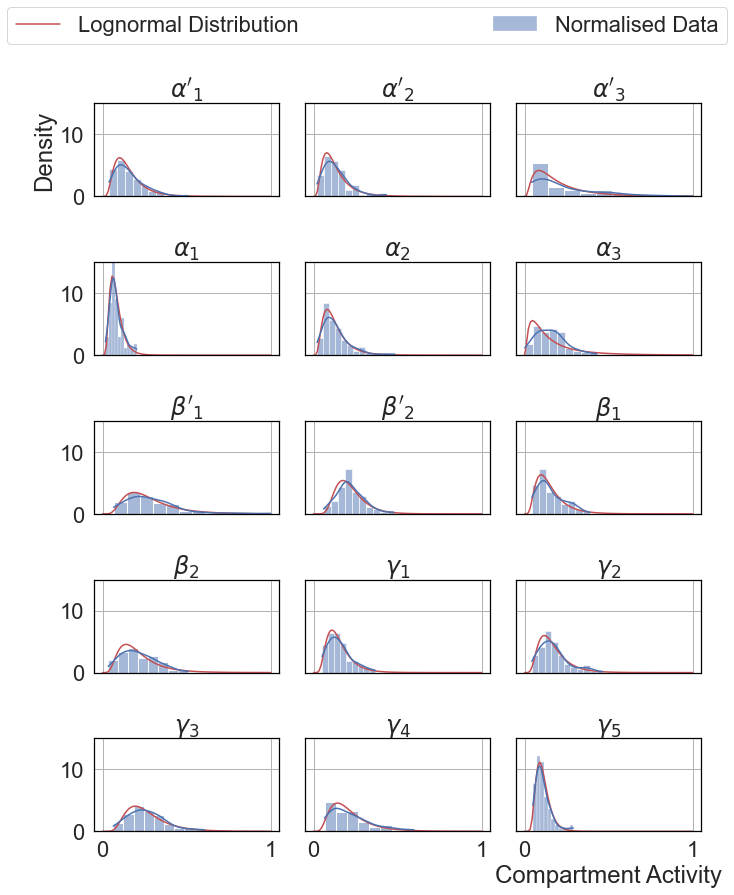
\includegraphics[width=\textwidth]{dan-distribution.png}
        		\caption{}
        		\label{fig:dan-distribution}
     	\end{subfigure}
     	\hfill
     	\begin{subfigure}[b]{0.49\textwidth}
         	\centering
         	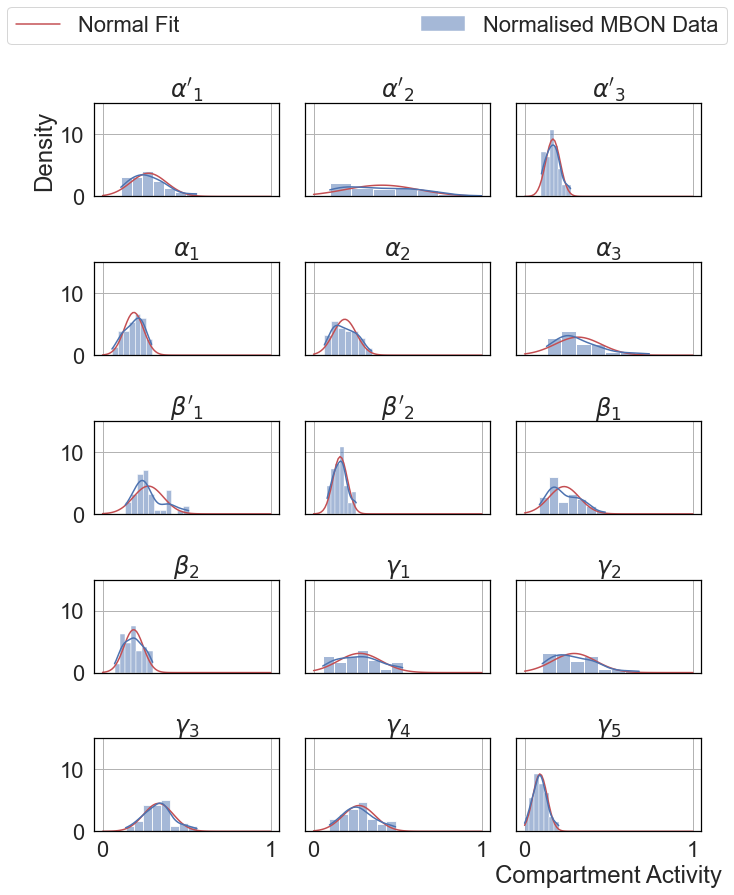
\includegraphics[width=\textwidth]{mbon-distribution.png}
        		\caption{}
         	\label{fig:mbon-distribution}
     	\end{subfigure}
	~
	\begin{subfigure}[b]{0.48\textwidth}
		\centering
        		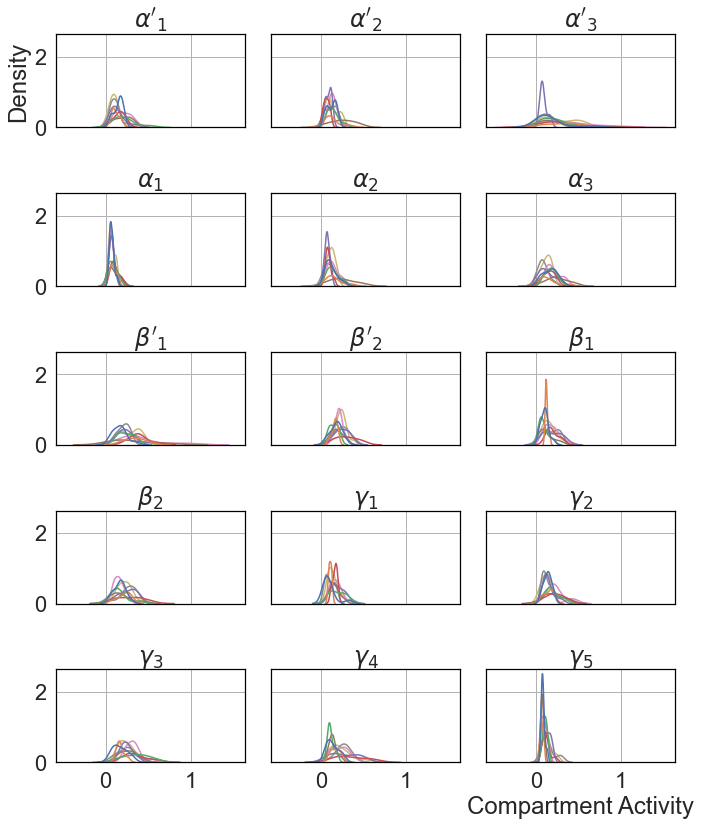
\includegraphics[width=\textwidth]{dan-distribution-all-stimuli.png}
        		\caption{}
        		\label{fig:dan-distribution-all-stimuli}
     	\end{subfigure}
     	\hfill
     	\begin{subfigure}[b]{0.48\textwidth}
         	\centering
         	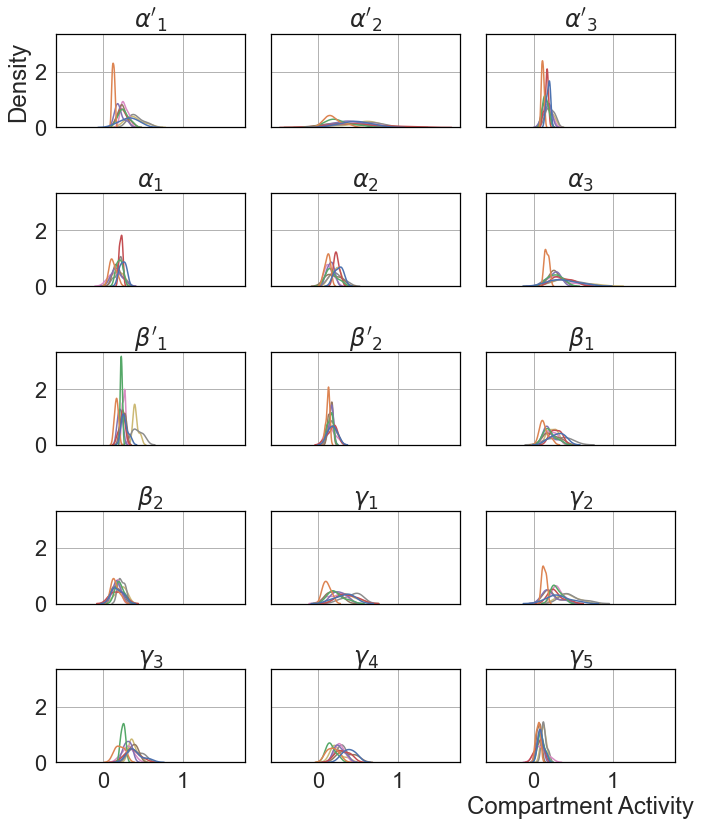
\includegraphics[width=\textwidth]{mbon-distribution-all-stimuli.png}
        		\caption{}
         	\label{fig:mbon-distribution-all-stimuli}
     	\end{subfigure}
	\caption{
	DAN data generally follows a lognormal distribution, where the MBON data can be modelled using a normal distribution. For distributions fitted to each of the compartment's activity across all stimuli:
	\textbf{(a)} shows that log-normal distribution fits DAN activity reasonably well; and
	\textbf{(b)} shows that normal distribution fits MBON activity reasonably well. You can then fit a distribution to each compartment for each stimulus as seen in 
	\textbf{(c)} for DAN data; and in
	\textbf{(d)} for MBON data.
	There are therefore 9 DAN distributions and 9 MBON distributions for every compartment.
	}
	\label{fig:data-distributions}
\end{figure*}


% ==== Simulate Calcium =====
\subsection{Simulating A Typical Calcium Response}

\begin{figure}[H]
	\centering
	\begin{subfigure}[b]{0.37\textwidth}
		\centering
        		\caption{}
        		\includegraphics[width=\textwidth]{dan-calcium-response.png}
        		\label{fig:dan-calcium-response}
     	\end{subfigure}
     	~
     	\begin{subfigure}[b]{0.36\textwidth}
         	\centering
        		\caption{}
         	\includegraphics[width=\textwidth]{dan-scaled-exponential.png}
         	\label{fig:dan-scaled-exponential}
     	\end{subfigure}
	\caption{
		(\textbf{a})  Mean of all the calcium traces in the Siju data. This is considered to be a baseline curve for the fluorescence signal.
		(\textbf{b})  Examples of generated DAN timeseries for train, test and validation datasets.
	}
\end{figure}


\begin{figure*}[t]
	\centering
  	\parbox{\textwidth}{
    	\parbox{.6\textwidth}{%
      		\subcaptionbox{}{
			\includegraphics[width=\hsize]{mbon-connectomics-cells.png}}
    	}
    	\hskip1em
    	\parbox{.3\textwidth}{%
      		\subcaptionbox{}{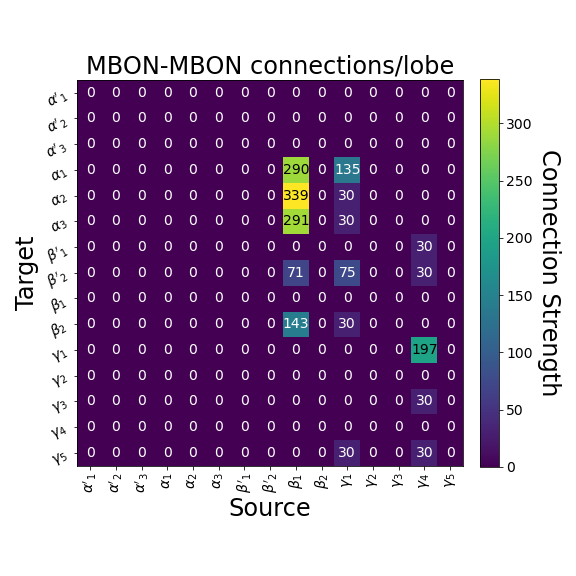
\includegraphics[width=\hsize]{mbon-connectomics-compartments.png}}
      		\subcaptionbox{}{\includegraphics[width=0.86\hsize]{mbon-mbon-mask.png}}  
    	}
  	}
 	 \caption{Connectomics data collected from \cite{li2020connectome}. 
	\textbf{(a)} connectomics data for the MBON to MBON feedforward network. The synapse counts are given if they found more than 30 synapses. 
	\textbf{(b)} A measure of inter-compartment connectivity in the feedforward MBON-MBON network. This is based on the synapse counts shows in (a). 
	\textbf{(c)} Masking matrix used to constrain optimisation of recurrent MBON connections. This mask is based on the known inter-compartment connections between MBONs.}
	\label{fig:mbon-connectomics}
\end{figure*}

Up until this point we have only considered scalar values which are used to quantify compartment activity. In both original experiments these scalars are calculated by averaging a time series. Both of the datasets were recorded using calcium imaging. The calcium levels detected in each frame are averaged to yield the final activity. 



Since, in the recurrent model, MBON activity is fed back to influence MBON activity at the following time step, the dataset needs to take time into account. Therefore, a logical choice is to model a typical 'calcium response' over time and convolve that baseline waveform with each sample taken from our data distributions. In this way the scalar activity values are transformed back into sequences in time. 

Since the full time series data is available, the DAN dataset is used to determine an appropriate waveform to be used as a template. The mean of the calcium imaging data is taken over all trials (see Figure \ref{fig:dan-calcium-response}). Unfortunately the sampling rate at which data was collected is not known.


The full calcium response data is not available for the MBON dataset. Therefore, it is assumed that the MBONs would respond with a similar rise and exponential decay as the DANs.

It is assumed that the exact shape of the curve is not important. A very simple baseline curve, based on the data seen in the DAN dataset, is therefore used. For each value in the train, test and validation datasets a time-series is generated by scaling the baseline curve to ensure that the mean of the resulting sequence is equivalent to the sampled value (which is itself a mean of the recorded calcium trace).

\begin{equation}
o(t) = b(t) \times \frac{s}{u}
\end{equation}

Where $o(t)$ is the output sequence with mean $u$; $b(t)$ is some baseline curve; and $s$ is a sample from the activity distribution.


% ==== Connectomics =====
\subsection{Connectomics Data}

To evaluate whether an optimised model correctly determines the connectivity between DANs and MBONs the learned parameters of the computational model are compared to the true synaptic strengths. 

This connectomics data from  \cite{li2020connectome} includes the number of synapses in the feedforward MBON-MBON circuit (see Figure \ref{fig:mbon-connectomics}a). It does not, however, specify the number of synapses between specific DANs and MBONs in the MB compartments.

Since the models in this investigation do not predict activity in MBON cell types, but rather in MBON compartments, the connectomics matrix is transformed using the same procedure and weightings used to transform Hige's MBON dataset from cell activities to compartment activities (see Figure \ref{fig:mbon-connectomics}b).



		

% ==== Models =====
\section{Modelling}
This Section presents several of feedforward models, increasing in complexity,  used to model the relationship between DANs and MBONs. In each of the models there are 15 DAN nodes which represent the DAN activity in each MB compartment, and 15 MB nodes which represent the MBON activity in those same compartments.


\begin{figure}[H]
	\centering
	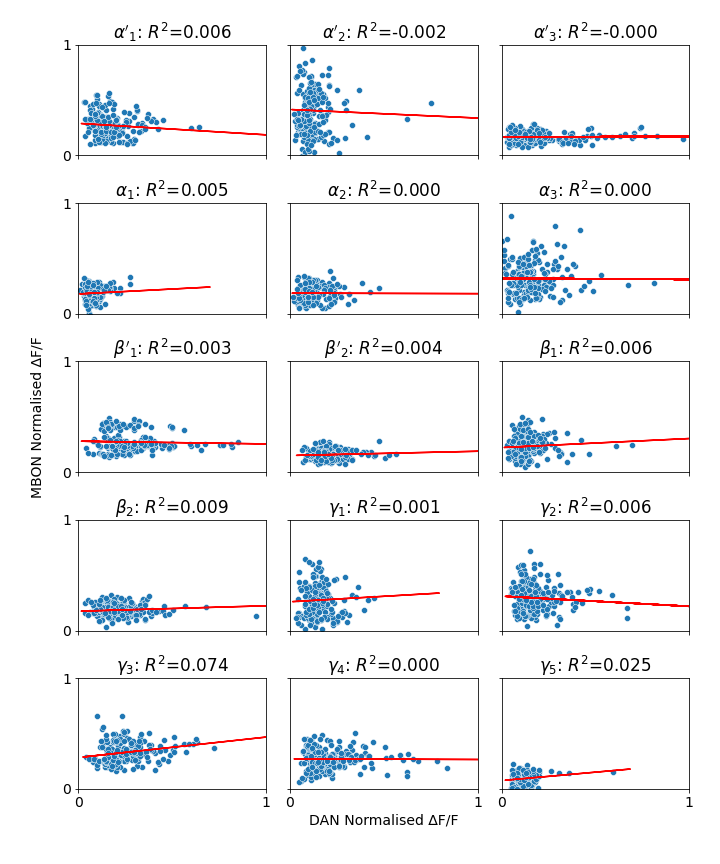
\includegraphics[width=\linewidth]{canonical-fit.png}
	\caption{Linear regression on the canonical model fitted to the training dataset}
	\label{fig:canonical-fit}
\end{figure}


% ==== Assumptions and Limitations ==== 
\subsection{Assumptions and Limitations}
A simplified circuit to investigate the relationship between DANs and MBONs is modelled using several approaches. The inputs to the model are DAN activity, and the output is the resulting MBON activity. Two critical simplifications are made:

\begin{enumerate}
\itemsep0em
\item
The inputs derived from KCs are not used
\item
Known sources of recurrence between MBONs and DANs are not taken into account
\end{enumerate}

This allows the model to more directly determine the feedforward effect of DAN activity on MBON activity. 

Each of the models is optimised using the available data. However, the amount of data is limited. Furthermore the MBON activity was collected in a separate experiment to the DAN activity in different sets of flies. An effort has been overcome these limitations.


		

% ==== Canonical Model=====
\subsection{Canonical Model}

Based on previous studies in the cellular anatomy of the MB \cite{li2020connectome, aso2014neuronal}, there are a small number of DAN cells which innervate each of the compartments. Many of DANs only innervate a single compartment. A one-to-one mapping from DAN compartment activity to MBON compartment activity is therefore the simplest model of the relationship between DANs and MBONs (see Figure \ref{fig:model-canonical}). In this model, activity is isolated in each compartment. 


Linear regression is used to fit this model to the 18000 training trials sampled from the MBON and DAN activity distributions (see Figure \ref{fig:canonical-fit}). Each compartment therefore has an associated weight and a bias which linearly transforms DAN activity to MBON activity. 

% ==== Cross Talk Model=====
\subsection{Linear Model with Cross Talk}
A more complex linear feedforward model disregards the canonical mapping between DANs and MBONs. Instead every DAN node has a feed forward connection to every MBON node (see Figure \ref{fig:model_dense_feedforward}). This allows for cross talk between the MB compartments. 


Once again Multivariate Linear Regression is used to fit this dense model to the training dataset. One would expect to see a strong diagonal in the connectivity matrix. However, after optimisation, the resulting weight matrix does not resemble the canonical model of the MB. Therefore, the model's connectivity does not reflect what is thought to be the underlying pattern of cellular connectivity. 

% ==== Naive Recurrent Model =====
\subsection{Naive Recurrent Model}

The previous models have ignored the fact that MBON cells form a feedforward network. These recurrent connections may be essential in predicting MBON activity. Taking this known recurrence into account one can build a naive recurrent model where every DAN compartment is allowed to feed forward to every MBON compartment, and each MBON compartment feeds back to every MBON compartment (see Figure \ref{fig:model-recurrent-overview}). 

% models
\begin{figure}[H]
	\centering
	\begin{subfigure}[b]{0.48\textwidth}
        		\caption{}	
		\centering	
        		\includegraphics[width=\textwidth]{model-canonical.png}
        		\label{fig:model-canonical}
     	\end{subfigure}
     	\vspace{1em}
     	\begin{subfigure}[b]{0.48\textwidth}
         	\centering
         	\caption{}
         	\includegraphics[width=\textwidth]{model_dense_feedforward.png}
         	\label{fig:model_dense_feedforward}
     	\end{subfigure}
	~
	\begin{subfigure}[b]{0.48\textwidth}
         	\centering
         	\caption{}
         	\includegraphics[width=\textwidth]{model-recurrent-detailed.png}
		\label{fig:model-recurrent-detailed}
     	\end{subfigure}
	~
	\begin{subfigure}[b]{0.48\textwidth}
		\centering
         	\caption{}
        		\includegraphics[width=\textwidth]{model-recurrent-overview.png}
		\label{fig:model-recurrent-overview}
     	\end{subfigure}
	\caption{Different models were used to optimise a fit between the DAN dataset and MBON dataset. 
	\textbf{(a)}  Canonical (one-to-one) model of DAN to MBON feedforward connectivity. Recurrent connections between MBONs are ignored. 
	\textbf{(b)}  Linear model with dense cross talk. Every DAN feeds forward its activity to every MBON.
	\textbf{(c)} Detailed view of the naive recurrent model.
	\textbf{(d)}  Overview of naive recurrent model where each MBON compartment feeds back its activity to every MBON compartment in the next time step.
	}
\end{figure}


% results: heat maps
\begin{figure*}
	\centering
	\begin{subfigure}[b]{0.46\textwidth}
		\centering
        		\caption{}
        		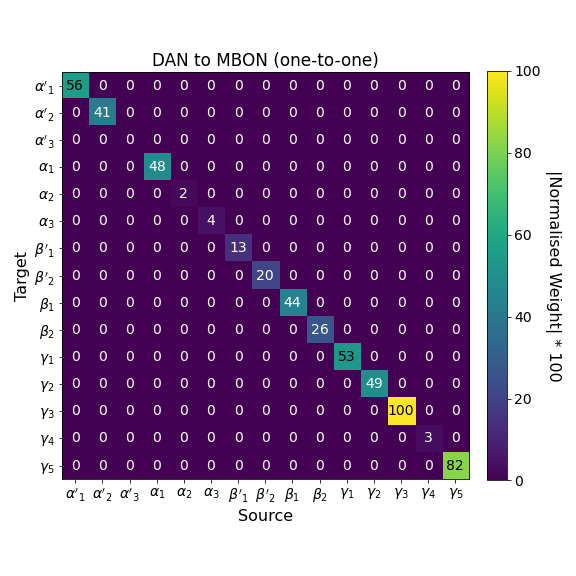
\includegraphics[width=\textwidth]{weights-dan-to-mbon-canonical.png}
        		\label{fig:weights-dan-to-mbon-canonical}
     	\end{subfigure}
     		\vspace{-0.9em}
     	\begin{subfigure}[b]{0.46\textwidth}
         	\centering
         	\caption{}
         	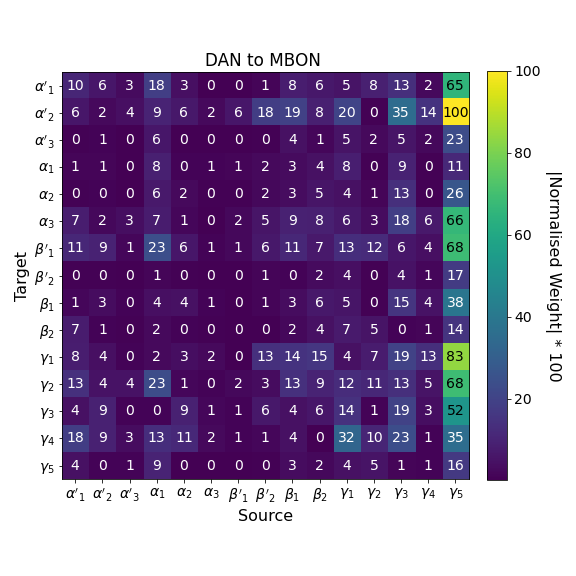
\includegraphics[width=\textwidth]{weights-dan-to-mbon-cross-talk.png}
         	\label{fig:weights-dan-to-mbon-cross-talk}
     	\end{subfigure}
	\vspace{-0.9em}
     	\begin{subfigure}[b]{0.46\textwidth}
         	\centering
         	\caption{}
         	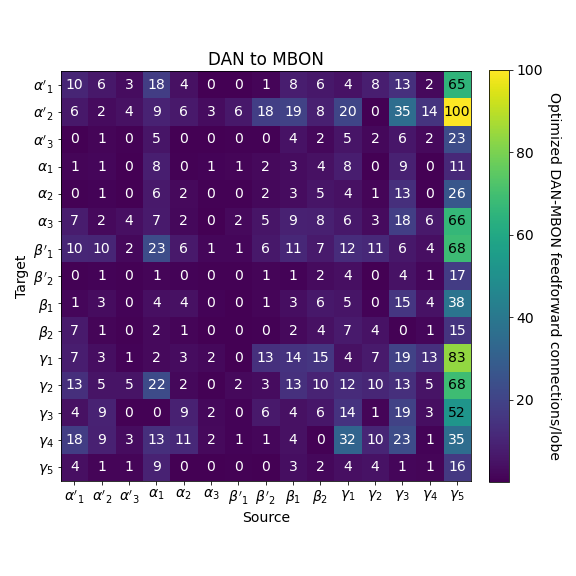
\includegraphics[width=\textwidth]{constrained_rnn_dan_mbon_matrix.png}
         	\label{fig:constrained_rnn_dan_mbon_matrix}
     	\end{subfigure}
	~
     	\begin{subfigure}[b]{0.46\textwidth}
         	\centering
         	\caption{}
         	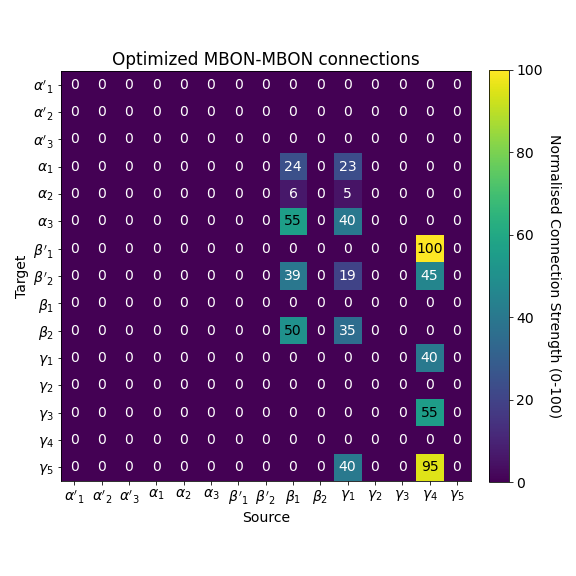
\includegraphics[width=\textwidth]{constrained_rnn_mbon_mbon_matrix.png}
         	\label{fig:constrained_rnn_mbon_mbon_matrix}
     	\end{subfigure}
	~
	\begin{subfigure}[b]{0.46\textwidth}
         	\centering
         	\caption{}
         	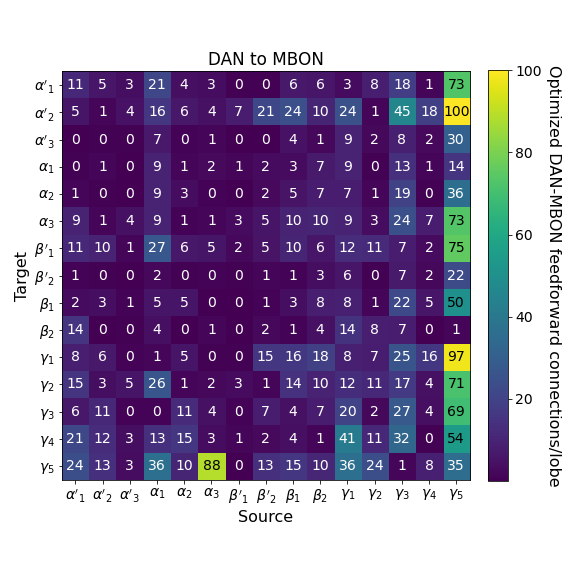
\includegraphics[width=\textwidth]{unconstrained_rnn_dan_mbon_matrix.png}
         	\label{fig:unconstrained_rnn_dan_mbon_matrix}
     	\end{subfigure}
	~
     	\begin{subfigure}[b]{0.46\textwidth}
         	\centering
         	\caption{}
         	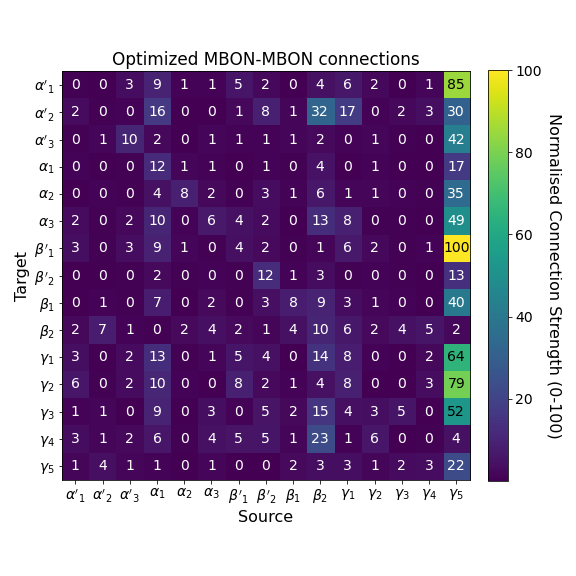
\includegraphics[width=\textwidth]{unconstrained_rnn_mbon_mbon_matrix.png}
         	\label{fig:unconstrained_rnn_mbon_mbon_matrix}
     	\end{subfigure}
		\vspace{-0.9em}
	\caption{
	Learned inter-compartment weightings between:
	\textbf{(a)} DANs and MBONs in the canonical model;
	\textbf{(b)} DANs and MBONs in the linear model with cross talk;
	\textbf{(c)} DANs and MBONs in the constrained recurrent model.
	\textbf{(d)} MBONs and MBONs in the constrained recurrent model.
	\textbf{(e)} DANs and MBONs in the naive recurrent model.
	\textbf{(f)}  MBONs and MBONs in the naive recurrent model.	
	}
\end{figure*}



This network is implemented as a 'vanilla' recurrent neural network (RNN) as shown in Figure \ref{fig:weights-dan-to-mbon-cross-talk}. The input features at each time step consist of the activity in each of the 15 DAN compartments. The output of the model is computed using these input features and the outputs from the previous time step. 

\begin{equation}
M_{(i,t)} = tanh(W_{hh} M_{(i,t-1)} + W_{xh} D_{(i,t)})
\end{equation}

Where:
\begin{itemize}
\item
$M_{(i,t)} \in \Re^{1\times15}$ is the MBON activity for sample $i$ at time $t$
\item
$M_{(i,t)} \in \Re^{1\times15}$ is the predicted MBON activity for sample $i$ at the previous time step $t-1$
\item
$D_{(i,t)} \in \Re^{1\times15}$ is the DAN activity for sample $i$ at time $t$
\item
$W_{xh}\in \Re^{15\times15}$ is the weight matrix which determines the effect of the input features on the output at every time step
\item
$W_{hh}\in \Re^{15\times15}$ is the weight matrix which determines the effect of the previous time step on the output at every time step 
\end{itemize}

The inputs of the training dataset will comprise of generated DAN time series such as the one shown in Figure \ref{fig:dan-scaled-exponential}. Each of these inputs contains 15 features (corresponding to the 15 compartments) and extends over ten time steps ($X_i \in \Re ^{10\times 15}$). Each time series and includes a short rise time and an exponential decay to emulate a typical fluorescence reading. The mean of each input time series is sampled from a distribution which models the average activity in a compartment for some given stimulus. 

The output of the network is not a time series but rather a scalar value representing the mean MBON activity ($Y_i \in \Re ^{1\times 15}$). Since the time series data for the MBONs is not available, generating a typical shape for the MBON fluorescence response is not possible. Therefore the RNN is not constrained in the response that it generates at each time-step. The only restriction is that imposed is on the mean of the generated MBON time-series. 

After allowing the model to find optimal weights for its feedforward and recurrent connections, the model is validated by comparing these weights to the connectome in Figure \ref{fig:mbon-connectomics}. 


		

% ==== Constrained Recurrent Model =====
\subsection{Constrained Recurrent Model}
Rather than hoping that the naive recurrent model converges to a weight matrix similar to the connectome of the MBON, one can constrain the recurrent model to only allow known connections between compartments. The masking matrix in Figure \ref{fig:mbon-connectomics}c is used to constrain the MBON to MBON recurrent connections in each forward pass of the model. Therefore, rather than allowing recurrent connections between all MBONs, only connections found by Li et al \cite{li2020connectome} are permitted. 

Following this logic, the connections between DANs and MBONs is also constrained. Rather than allowing each DAN compartment to effect every MBON compartment, the feedforward layer from DANs-MBONs is constrained along the diagonal of the connectivity matrix (identical to the simple linear model used  in the Canonical Model). This mapping is a better fit to the known anatomy of the MB. 


The linear layers of the naive RNN are constrained by multiplying the learned weights with a masking matrix during each forward pass. Therefore, the strength of the permitted connections between the model's nodes are still learned using back propagation. These weights can then be compared to the inter-compartment connectivity matrix in Figure \ref{fig:mbon-connectomics}b.


\begin{figure*}[t]
	\centering
	\begin{subfigure}[b]{0.32\textwidth}
         	\centering
         	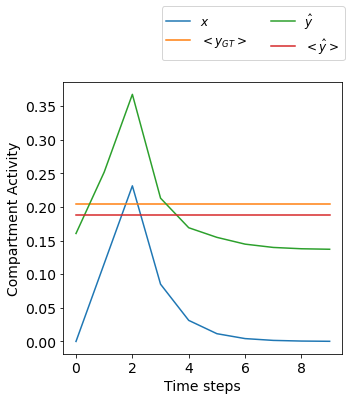
\includegraphics[width=\textwidth]{recurrent-predicted-activity.png}
         	\caption{}
         	\label{fig:recurrent-predicted-activity}
     	\end{subfigure}
	\hfill
	\begin{subfigure}[b]{0.32\textwidth}
		\centering
        		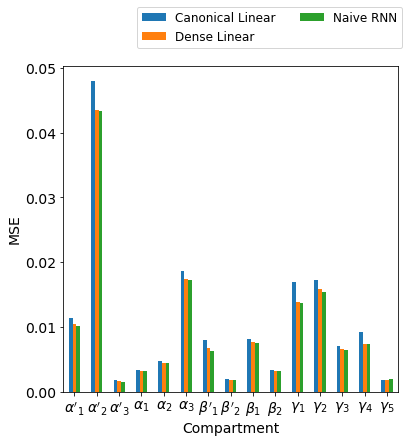
\includegraphics[width=\textwidth]{comparison-mse-naive.png}
        		\caption{}
        		\label{fig:comparison-mse-naive}
     	\end{subfigure}
	\hfill
	\begin{subfigure}[b]{0.32\textwidth}
		\centering
        		\includegraphics[width=\textwidth]{comparison-r2-naive.png}
        		\caption{}
        		\label{fig:comparison-r2-naive}
     	\end{subfigure}
     	\hfill
	\begin{subfigure}[b]{0.32\textwidth}
		\centering
        		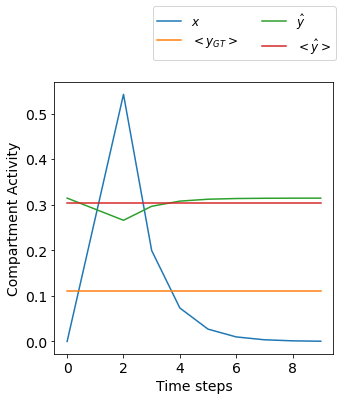
\includegraphics[width=\textwidth]{masked-recurrent-predicted-activity.png}
        		\caption{}
        		\label{fig:masked-recurrent-predicted-activity}
     	\end{subfigure}
     	\hfill
	\begin{subfigure}[b]{0.32\textwidth}
		\centering
        		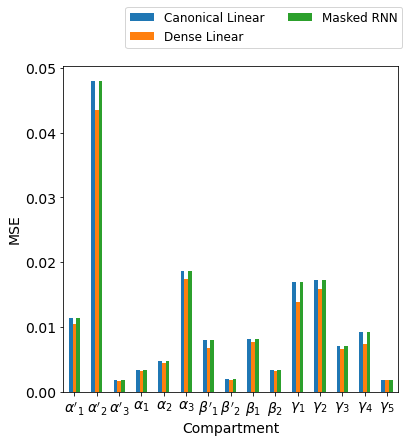
\includegraphics[width=\textwidth]{comparison-mse-masked.png}
        		\caption{}
        		\label{fig:comparison-mse-masked}
     	\end{subfigure}
     	\hfill
	\begin{subfigure}[b]{0.32\textwidth}
		\centering
        		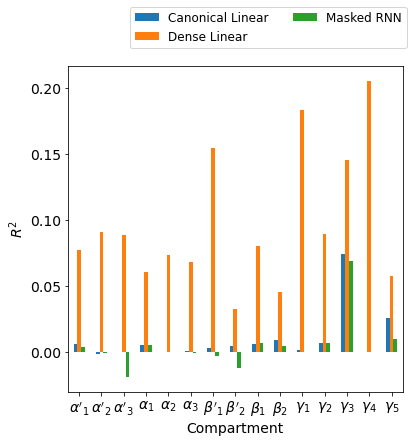
\includegraphics[width=\textwidth]{comparison-r2-masked.png}
        		\caption{}
        		\label{fig:comparison-r2-masked}
     	\end{subfigure}
	\caption{Different representations of the model's ability to fit the data.
		\textbf{(a)} MBON activity predicted by the naive recurrent model shown as the generated time series $\hat y$ and its mean $<\hat y >$. This is plotted with the input DAN time series $x$, and the ground truth MBON mean activity $<y_{GT}>$.
		\textbf{(b)} MSE comparison between $<y_{GT}>$ and $<\hat y >$ in the testing set for both linear models and the naive recurrent model.
		\textbf{(c)} $R^2$ fitting parameter for both linear models and the naive recurrent model.
		\textbf{(d)} MBON activity predicted by the constrained recurrent model
		\textbf{(e)} MSE comparison between $<y_{GT}>$ and $<\hat y >$ in the testing set for both linear models and the masked recurrent model.
		\textbf{(f)}	$R^2$ fitting parameter for both linear models and the masked recurrent model.	
	}
\end{figure*}


% ==== Results and discussion =====
\section{Results and Discussion}

After fitting the four models to the data they can be evaluated in two ways. First, the MSE and $R^2$ for each of the models is compared using the same testing dataset (4500 data points). Secondly, the learned inter-compartment weights are compared to the known connectomics.

\subsection{Fitting the dataset}
As seen in Figure \ref{fig:comparison-mse-naive}, the MSE error between the canonical linear, dense linear and naive recurrent model all converge to a similar value. However the dense model consistently achieves the lowest loss. Although the recurrent model on average achieves a lower loss than the canonical linear model, their results are comparable. The ``goodness of fit" between these same three models is compared in Figure \ref{fig:comparison-r2-naive}. According to this metric, the recurrent model performs extremely poorly and in many cases predicting the mean of the input data would be more accurate (indicated by negative $R^2$). 

An identical comparison is conducted between the constrained recurrent model and the two linear models. Figure \ref{fig:comparison-mse-masked} shows that, despite increased model complexity, the constrained model does achieve a lower MSE than either of the linear models. Similarly, although not as poor as the naive model, the masked model attains extremely low, and often negative $R^2$ scores (see Figure  \ref{fig:comparison-r2-masked}).

\subsection{Predicting the connectome}
Both linear models only learned weight matrices to relate DAN activity to MBON activity. Unfortunately, to the authors knowledge, no connectomics data between DAN and MBON cells is available as a reference point. However, one should expect a predominant feature along the diagonal. This diagonal is imposed by the canonical model (see Figure \ref{fig:weights-dan-to-mbon-canonical}, but in the densely connected linear model this diagonal nature does not emerge during optimisation. This can be seen in  Figure \ref{fig:weights-dan-to-mbon-cross-talk} where the weights are disproportionately high from $\gamma 5$ to the other compartments. This may be the network compensating for consistently lower DAN activity in the $\gamma 5$ compartment (see Figure \ref{fig:siju-activity-per-stim}). 

Ideally the unconstrained `naive' recurrent model would have been able to capture this diagonal connectivity mapping form DAN-MBONs as well as converge to the recurrent connections found via a connectomics analysis of the MB. However, after 20 epochs training on the 18000 training time-series, the model's weights do not resemble these underlying patterns of connectivity. In fact the learned weights do not display any structure (see Figures \ref{fig:unconstrained_rnn_dan_mbon_matrix}, \ref{fig:unconstrained_rnn_mbon_mbon_matrix}). This is not surprising since, given limited data, there are sure to be many local minima on the model's loss manifold. Even if one of those minima resembles the connectome, the high dimensionality of the space means it is unlikely that the network will find and converge to that optimal point. 

To circumvent this problem the RNN weight matrix was constrained by the connectome. Only the known connections between compartments could be learned by this model. Figure \ref{fig:constrained_rnn_dan_mbon_matrix} shows the learned weights along the imposed diagonal DAN-MBON connectivity matrix. This mapping is not significantly similar to the weightings learned by the canonical model. Furthermore, the learned recurrent weights from MBONs MBONs do not resemble the connectome (see Figure \ref{fig:constrained_rnn_mbon_mbon_matrix}).


\section{Conclusions and Future Work}
Unfortunately, none of the models explored exposed the underlying connectome. Furthermore the models fit to the data was lower than expected. This could be due to the nature of the datasets. According to \cite{hige2015} the activity of MBONs is unique to every fly. The tuning of these cell's responses to certain odours is not shared across animals. Therefore, it may be that the DAN activity which affect the MBONs is also unique. An attempt to predict MBON data from DAN data where each dataset are recorded in unrelated populations of flies may not be possible. This could explain the low $R^2$ values.

However, if making this kind of prediction is in fact possible, the results remain highly dependent on the data that is ultimately used to train the models. There are several improvements that can be made to ensure higher quality training data. Access to the time dependent calcium imaging readouts from \cite{hige2015} could be used to generate a generic time series for the MBON responses. This could be used to train a RNN where the output at each time step would aim to match that of the ground truth MBON response. 

Furthermore, many assumptions were made when generating the dataset. For example, the mapping from MBON cell types to compartments could have introduced artefacts that the model could not account for. It is recommended that these assumptions be revised, and that the number of cells in each of the lobes is included in the mapping from cells to compartments.

A different approach altogether would be to simply predict the activity in each of the MBONs. The number of MBONs is scarcely more than the number of MB compartments. Using the DAN acitivty in each compartment to predict the MBON responses at a cellular level may prove more effective. This would also allow the model to take the type of neurotransmitter that the MBON releases into account. In this kind of analysis the fact that DANs release dopamine, rather than simply being modelled as generic neurons, may play a role. 

Lastly, it is clear that recurrence from MBONs to DANs is an important component of the MB circuit \cite{li2020connectome}. Taking these connections into account may be essential. 

% take the MBON-DAN recurrence into account

% ==== Bibliography =====
\bibliographystyle{apalike}
\bibliography{mushroom_body.bib}
 
\end{multicols}

% ---------------------------------------------------------------------------------------------------------------------------------------------------
% APPENDIX
% ---------------------------------------------------------------------------------------------------------------------------------------------------

\newpage
\clearpage
\section*{APPENDIX}
\setcounter{page}{1}
\renewcommand{\thepage}{\roman{page}}
\appendix
\setcounter{figure}{0} 	%figures start counting from zero again
\renewcommand\thefigure{\thesection.\arabic{figure}} 	% makes the numbers appear as Figure A.1:
\setcounter{table}{0} 		%tables start counting from zero again
\renewcommand\thetable{\thesection.\arabic{table}} 

\section{Dataset Visualisations}

\begin{figure}[H]
	\centering
	\includegraphics[width=\linewidth]{siju-activity-per-stim.png}
	\caption{Siju 2020 recorded DAN activity in each of the 15 compartments for each of the nine shared stimuli.}
	\label{fig:siju-activity-per-stim}
\end{figure}

\begin{figure}[H]
	\centering
	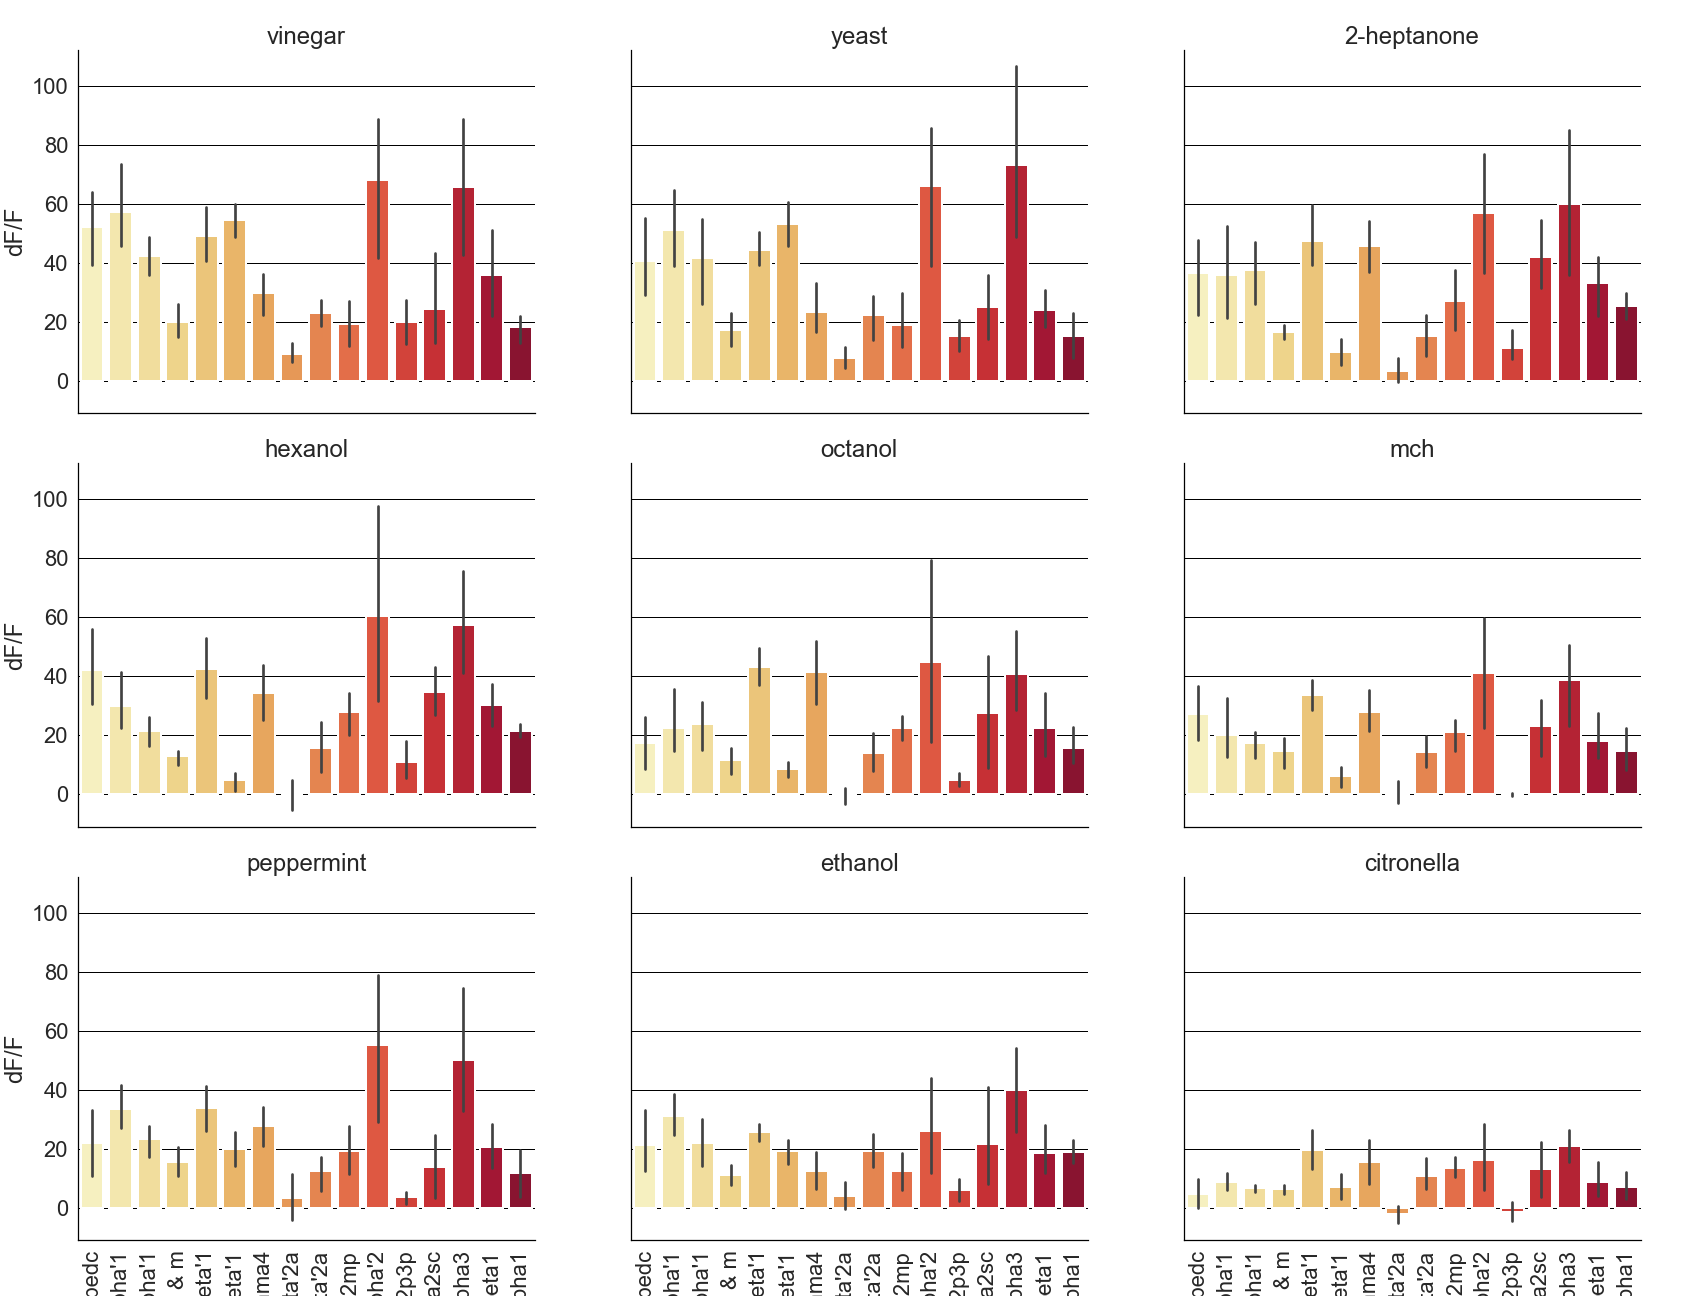
\includegraphics[width=\linewidth]{hige-activity-per-stim.png}
	\caption{Hige 2014 recorded MBON activity in each 16 cell types and 2 combinations for each of the nine shared stimuli.}
	\label{fig:hige-activity-per-stim}
\end{figure}

\newpage

\section{Cell to Compartment Mapping}

\begin{figure}[H]
	\centering
	\includegraphics[width=0.73\textwidth]{aso_cell_to_compartment.jpg}
	\caption{Distribution of MBON cell types, DAN cell types and KC cell types in the MB compartments taken from \cite{aso2014neuronal}.}
	\label{fig:mbons_per_lobe}
\end{figure}








% ----------------------------------------------------------------------------------------------------------------------------------
% End Document
% ----------------------------------------------------------------------------------------------------------------------------------
\end{document}